\chapter{Relevante Concepten}\label{ch:concepten}

In dit hoofdstuk leggen we alle concepten uit die nodig zijn om de volledige functionaliteit van de webapp te begrijpen.

Dit hoofdstuk is hoofdzakelijk gebaseerd op ~\cite{LightingTechnologyHandbook,InteriorLightingHandbook,Light-EmittingDiodes,FundamentalsofSolidStateLighting}

\section{Spectral power distribution}{\label{sec:spectral-power-distribution}}

De \gls{spd} is een essentieel concept voor het gebruik van de app en de verschillende berekeningen die hierin worden uitgevoerd. Het vormt de basis voor alle andere berekeningen. Bovendien maakt de \gls{spd} het eenvoudig om experimentele aanpassingen snel te visualiseren. Aan de hand van de \gls{spd} kunnen we per golflengte zien hoeveel optische straling wordt uitgezonden. Het wordt gedefinieerd als de hoeveelheid optische straling die door een bron wordt uitgezonden binnen een smalle band $\Delta\lambda$, gecentreerd rond een specifieke golflengte $\lambda$. Door een grafiek van de spectral power distribution te maken, kunnen we bijvoorbeeld zien bij welke golflengte een \gls{led} de grootste optische straling heeft en welk effect het toevoegen van luminescente materialen heeft.

\begin{figure}[H]
    \centering
    \resizebox{0.7\textwidth}{!}{% This file was created with tikzplotlib v0.10.1.
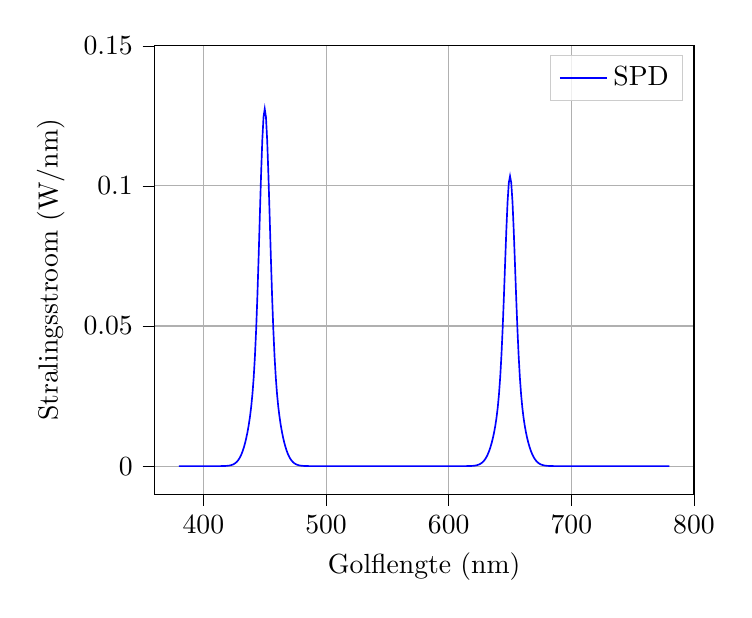
\begin{tikzpicture}

\definecolor{darkgray176}{RGB}{176,176,176}
\definecolor{lightgray204}{RGB}{204,204,204}

\begin{axis}[
legend cell align={left},
legend style={fill opacity=0.8, draw opacity=1, text opacity=1, draw=lightgray204},
tick align=outside,
tick pos=left,
x grid style={darkgray176},
xlabel={Golflengte (nm)},
xmajorgrids,
xmin=360, xmax=800,
xtick style={color=black},
y grid style={darkgray176},
ylabel={Stralingsstroom (W/nm)},
ymajorgrids,
ymin=-0.01, ymax=0.15,
yticklabels={-0.01, 0, 0.05, 0.1, 0.15},
ytick style={color=black}
]
\addplot [semithick, blue]
table {%
380 1.02073728218891e-15
381 2.48463356981015e-15
382 5.9710643336564e-15
383 1.41671399063567e-14
384 3.31859034825859e-14
385 7.67478360943115e-14
386 1.75234520140434e-13
387 3.95015573955344e-13
388 8.79123327229562e-13
389 1.9316410234851e-12
390 4.19028986979639e-12
391 8.97434465598681e-12
392 1.89759030340542e-11
393 3.96134977666599e-11
394 8.16441290421166e-11
395 1.66129883456256e-10
396 3.33742558513386e-10
397 6.61936687321886e-10
398 1.29617112990747e-09
399 2.5058165109343e-09
400 4.78274492556851e-09
401 9.01251920821373e-09
402 1.67670329461642e-08
403 3.07969184267533e-08
404 5.58469343871304e-08
405 9.99844460004153e-08
406 1.76728495979833e-07
407 3.08405240440691e-07
408 5.3134665042051e-07
409 9.03805908085318e-07
410 1.51779610976949e-06
411 2.51647560939047e-06
412 4.11920158656256e-06
413 6.65693624151611e-06
414 1.06212780781283e-05
415 1.67309342278416e-05
416 2.60198408056627e-05
417 3.99512257927416e-05
418 6.05614986236792e-05
419 9.06367132931326e-05
420 0.000133922242960297
421 0.000195362997908766
422 0.000281366856992435
423 0.000400077936995756
424 0.000561639068050377
425 0.00077841482796926
426 0.00106513852909163
427 0.00143893996057875
428 0.00191920760002315
429 0.00252724323990337
430 0.00328568613450886
431 0.00421773351462523
432 0.00534629488383525
433 0.0066934389805901
434 0.00828088606531231
435 0.0101328895377022
436 0.0122835132371137
437 0.0147905861658002
438 0.0177575796773932
439 0.0213610811858614
440 0.0258747153599907
441 0.0316715457905161
442 0.0391807935798618
443 0.0487787235769689
444 0.0606145246750115
445 0.0744090729810278
446 0.0893035494803108
447 0.103850903364327
448 0.116213345545371
449 0.124551928022846
450 0.1275
451 0.124551928022846
452 0.116213345545371
453 0.103850903364327
454 0.0893035494803108
455 0.0744090729810278
456 0.0606145246750115
457 0.0487787235769689
458 0.0391807935798618
459 0.0316715457905161
460 0.0258747153599907
461 0.0213610811858614
462 0.0177575796773932
463 0.0147905861658002
464 0.0122835132371137
465 0.0101328895377022
466 0.00828088606531231
467 0.0066934389805901
468 0.00534629488383525
469 0.00421773351462523
470 0.00328568613450886
471 0.00252724323990337
472 0.00191920760002315
473 0.00143893996057875
474 0.00106513852909163
475 0.00077841482796926
476 0.000561639068050377
477 0.000400077936995756
478 0.000281366856992435
479 0.000195362997908766
480 0.000133922242960297
481 9.06367132931326e-05
482 6.05614986236792e-05
483 3.99512257927416e-05
484 2.60198408056627e-05
485 1.67309342278416e-05
486 1.06212780781283e-05
487 6.65693624151611e-06
488 4.11920158656256e-06
489 2.51647560939047e-06
490 1.51779610976949e-06
491 9.03805908085318e-07
492 5.3134665042051e-07
493 3.08405240440691e-07
494 1.76728495979833e-07
495 9.99844460004153e-08
496 5.58469343871304e-08
497 3.07969184267533e-08
498 1.67670329461642e-08
499 9.01251920821373e-09
500 4.78274492556851e-09
501 2.5058165109343e-09
502 1.29617112990747e-09
503 6.61936687321886e-10
504 3.33742558513386e-10
505 1.66129883456256e-10
506 8.16441290421166e-11
507 3.96134977666599e-11
508 1.89759030340542e-11
509 8.97434465598681e-12
510 4.19028986979639e-12
511 1.9316410234851e-12
512 8.79123327229562e-13
513 3.95015573955344e-13
514 1.75234520140434e-13
515 7.67478360943115e-14
516 3.31859034825859e-14
517 1.41671399063567e-14
518 5.9710643336564e-15
519 2.48463356981015e-15
520 1.02073728218891e-15
521 4.14006001808021e-16
522 1.65783127084198e-16
523 6.55412995118465e-17
524 2.55817823406707e-17
525 9.85797202853517e-18
526 3.75046739484557e-18
527 1.40871856334676e-18
528 5.22401134581402e-19
529 1.91260380780255e-19
530 6.91332464117623e-20
531 2.46711797298917e-20
532 8.69228412377663e-21
533 3.02356243317445e-21
534 1.0383529437434e-21
535 3.52056272826524e-22
536 1.17847454399517e-22
537 3.89465825401622e-23
538 1.27074829524738e-23
539 4.09346184454742e-24
540 1.30185611745346e-24
541 4.08767407257552e-25
542 1.26715739841099e-25
543 3.87816160492372e-26
544 1.17182385798815e-26
545 3.49575211123742e-27
546 1.02960506615758e-27
547 2.99488653307453e-28
548 8.63614143122872e-29
549 2.58876117231654e-29
550 1.23493438572245e-29
551 2.16568468807202e-29
552 7.02803073593441e-29
553 2.43161485622973e-28
554 8.35809593355053e-28
555 2.83773147575922e-27
556 9.51245334716413e-27
557 3.14815473640599e-26
558 1.02863365337891e-25
559 3.31822954140463e-25
560 1.05680084828914e-24
561 3.32292785028049e-24
562 1.03154861614201e-23
563 3.16154611208376e-23
564 9.56644041596078e-23
565 2.85786856765061e-22
566 8.42898271979936e-22
567 2.45442126928279e-21
568 7.05608946518338e-21
569 2.00271929572062e-20
570 5.61199294401365e-20
571 1.55258426751031e-19
572 4.24066803366079e-19
573 1.14354801024619e-18
574 3.04449706169817e-18
575 8.00235376434031e-18
576 2.0766388017721e-17
577 5.32041137213813e-17
578 1.34576891397761e-16
579 3.36075460291217e-16
580 8.28598499659234e-16
581 2.01693783902236e-15
582 4.84709928261519e-15
583 1.15003841592778e-14
584 2.69391451799815e-14
585 6.23011845942058e-14
586 1.42249198702234e-13
587 3.20659701210809e-13
588 7.13641289162821e-13
589 1.56803800729967e-12
590 3.40152942371707e-12
591 7.285056250154e-12
592 1.5403968345291e-11
593 3.21568393635239e-11
594 6.62758223988946e-11
595 1.34858375982137e-10
596 2.70920429852043e-10
597 5.3733684029659e-10
598 1.05218597604254e-09
599 2.03413340299373e-09
600 3.88246352781444e-09
601 7.31604500431467e-09
602 1.36108855680627e-08
603 2.49998514287762e-08
604 4.53345702672e-08
605 8.11638444003371e-08
606 1.434619555601e-07
607 2.50352489298914e-07
608 4.31328457400179e-07
609 7.33677737151611e-07
610 1.23209331263641e-06
611 2.04278608291697e-06
612 3.34382246438607e-06
613 5.4038658901719e-06
614 8.62197867518649e-06
615 1.35815819026009e-05
616 2.11219884187144e-05
617 3.24309950552843e-05
618 4.91616871180454e-05
619 7.35756849085429e-05
620 0.00010871335016777
621 0.000158588786537704
622 0.000228403683911506
623 0.000324769148855378
624 0.000455918772887953
625 0.000631889683880929
626 0.000864641864792028
627 0.00116808067388157
628 0.00155794499295996
629 0.00205152686533332
630 0.00266720403860131
631 0.00342380720598989
632 0.00433993349393685
633 0.0054334975254202
634 0.00672213104125353
635 0.00822552209531119
636 0.00997132251012758
637 0.0120064758287084
638 0.0144149764440015
639 0.0173401717861699
640 0.0210041807039924
641 0.0257098430534777
642 0.0318055853765937
643 0.0395968461977747
644 0.0492047317950094
645 0.0604026592434226
646 0.0724934695781347
647 0.0843024980251592
648 0.0943378922662423
649 0.101106859218545
650 0.1035
651 0.101106859218545
652 0.0943378922662423
653 0.0843024980251592
654 0.0724934695781347
655 0.0604026592434226
656 0.0492047317950094
657 0.0395968461977747
658 0.0318055853765937
659 0.0257098430534777
660 0.0210041807039924
661 0.0173401717861699
662 0.0144149764440015
663 0.0120064758287084
664 0.00997132251012758
665 0.00822552209531119
666 0.00672213104125353
667 0.0054334975254202
668 0.00433993349393685
669 0.00342380720598989
670 0.00266720403860131
671 0.00205152686533332
672 0.00155794499295996
673 0.00116808067388157
674 0.000864641864792028
675 0.000631889683880929
676 0.000455918772887953
677 0.000324769148855378
678 0.000228403683911506
679 0.000158588786537704
680 0.00010871335016777
681 7.35756849085429e-05
682 4.91616871180454e-05
683 3.24309950552843e-05
684 2.11219884187144e-05
685 1.35815819026009e-05
686 8.62197867518649e-06
687 5.4038658901719e-06
688 3.34382246438607e-06
689 2.04278608291697e-06
690 1.23209331263641e-06
691 7.33677737151611e-07
692 4.31328457400179e-07
693 2.50352489298914e-07
694 1.434619555601e-07
695 8.11638444003371e-08
696 4.53345702672e-08
697 2.49998514287762e-08
698 1.36108855680627e-08
699 7.31604500431467e-09
700 3.88246352781444e-09
701 2.03413340299373e-09
702 1.05218597604254e-09
703 5.3733684029659e-10
704 2.70920429852043e-10
705 1.34858375982137e-10
706 6.62758223988946e-11
707 3.21568393635239e-11
708 1.5403968345291e-11
709 7.285056250154e-12
710 3.40152942371707e-12
711 1.56803800729967e-12
712 7.13641289162821e-13
713 3.20659701210809e-13
714 1.42249198702234e-13
715 6.23011845942058e-14
716 2.69391451799815e-14
717 1.15003841592778e-14
718 4.84709928261519e-15
719 2.01693783902236e-15
720 8.28598499659234e-16
721 3.36075460291217e-16
722 1.34576891397761e-16
723 5.32041137213813e-17
724 2.0766388017721e-17
725 8.00235376434031e-18
726 3.04449706169817e-18
727 1.14354801024619e-18
728 4.24066803366079e-19
729 1.55258426751031e-19
730 5.61199294401365e-20
731 2.00271929572062e-20
732 7.05608946518338e-21
733 2.45442126928279e-21
734 8.42898271979936e-22
735 2.85786856765061e-22
736 9.56644041596078e-23
737 3.16154611208374e-23
738 1.03154861614195e-23
739 3.32292785027808e-24
740 1.05680084827921e-24
741 3.31822954100161e-25
742 1.02863365176276e-25
743 3.14815467242237e-26
744 9.51245084624862e-27
745 2.83772182480431e-27
746 8.35772824290086e-28
747 2.43023181248878e-28
748 6.97667011378765e-29
749 1.97737803397955e-29
750 5.5331475723928e-30
751 1.52860695675071e-30
752 4.16927403308985e-31
753 1.12270609559045e-31
754 2.98478292084364e-32
755 7.83430458099105e-33
756 2.0301549371465e-33
757 5.19396412834549e-34
758 1.31192720744546e-34
759 3.27161026619249e-35
760 8.05479360303098e-36
761 1.95789005890491e-36
762 4.69854311830356e-37
763 1.113215290091e-37
764 2.60397097723442e-38
765 6.01359459342634e-39
766 1.37111279851383e-39
767 3.08640741245433e-40
768 6.85921399929498e-41
769 1.50499993921338e-41
770 3.26016546688947e-42
771 6.97242472027366e-43
772 1.47220760121888e-43
773 3.06898883240684e-44
774 6.31629770153123e-45
775 1.28342621172719e-45
776 2.57466215297901e-46
777 5.09930071577513e-47
778 9.97107606827849e-48
779 1.92492789283254e-48
780 3.66883290430096e-49
};
\addlegendentry{SPD}
\end{axis}

\end{tikzpicture}
}
    \caption{Voorbeeld spectral power distribution}
    \label{fig:VBSPD}
\end{figure}

\section{External quantum efficiency}{\label{sec:external-quantum-efficiency}}

Het volgende belangrijke concept is de \gls{eqe}. Dit begrip geeft aan hoeveel fotonen er voor de inkomende elektronen de \gls{led} verlaten. Dit is cruciaal bij het berekenen van de spectral power distribution van een \gls{led}. Afhankelijk van de centrale golflengte kan de external quantum efficiency namelijk sterk vari\"eren. Dit zorgt ervoor dat de hoeveelheid stralingsstroom voor bepaalde \gls{led}s een stuk kleiner is, doordat minder fotonen de \gls{led} kunnen verlaten. Zo hebben bijvoorbeeld groene \gls{led}s een veel lagere effici\"entie dan andere \gls{led}s (the green gap ~\cite{ExternalQuantumEfficiency,hahnClosingGreenGapb,FrontiersEQE,zhuSolidStateLightingBased2016EQE}), wat ervoor zorgt dat deze \gls{led}s meer vermogen nodig hebben. Het effect van de \gls{eqe} is rechtstreeks af te lezen in de spectral power distribution. Zo zal een groene \gls{led} met hetzelfde ingangsvermogen als een blauwe \gls{led} minder licht produceren.

\section{Chromaticiteit}\label{sec:chromaticiteit}

Door de verschillende \gls{spd}s van lichtbronnen ontstaat voor de mens een bepaalde kleur. Om te bepalen met welke kleur een \gls{spd} overeenkomt, maken we gebruik van een chromaticiteitsdiagram. Dit diagram helpt ons de kleur te visualiseren die wordt waargenomen op basis van de \gls{spd} van een lichtbron. Om op het chromaticiteitsdiagram tot een kleur te komen, moeten we eerst gebruik maken van de $\bar{x}(\lambda), \, \bar{y}(\lambda), \, \text{en} \, \bar{z}(\lambda)$ \gls{cmf} en de X, Y en Z tristimuluswaarden.

De \gls{cmf} (colour matching functions) zijn numerieke waarden die de chromatische respons van de waarnemer beschrijven. Chromatische respons betekent de manier waarop het menselijk oog verschillende golflengten van licht (kleuren) waarneemt. Het menselijk oog is namelijk gevoelig voor verschillende golflengtes, en de \gls{cmf} geven aan hoe sterk het oog reageert op licht bij verschillende golflengtes. Dit zijn als het ware de "gevoeligheidsfuncties" voor de verschillende kleuren die we kunnen waarnemen.

De X, Y en Z tristimuluswaarden zijn net zoals de RGB-waarden (rood, groen, blauw) een manier om een kleur voor te stellen, maar ze zijn gebaseerd op hoe een gemiddeld menselijk oog reageert op licht. De tristimuluswaarden X, Y en Z geven een gestandaardiseerde manier om de kleur van een lichtbron te berekenen op basis van de waarneming van de mens.

De waarnemer die we gebruiken om de \gls{cmf} te berekenen, is gebaseerd op de chromatische respons van een gemiddelde mens, die een respons heeft binnen een boog van twee graden van het gezichtsveld. Dit model wordt gebruikt omdat het menselijk zicht niet overal in het gezichtsveld even gevoelig is voor kleur. De \gls{cmf}s kunnen we dan zien als de spectrale "intensiteit" curves van drie lichtdetectoren, die samen de CIE-tristimuluswaarden X, Y en Z opleveren.

Aan de hand van de \gls{cmf} en de \gls{spd} van de te analyseren lichtbron kunnen we de X, Y en Z waarden berekenen op de volgende manier ~\cite{LightingTechnologyHandbook, CIE1931ColorSpace2024}:

\begin{align*}
X &= k.\int_{\lambda} \bar{x}(\lambda) P(\lambda) \, d\lambda \\
Y &= k.\int_{\lambda} \bar{y}(\lambda) P(\lambda) \, d\lambda \\
Z &= k.\int_{\lambda} \bar{z}(\lambda) P(\lambda) \, d\lambda
\end{align*}

Met $P(\lambda)$ de \gls{spd} van de lichtbron en $k$ een normalisatieconstante.

Aan de hand van deze tristimulus waarden kunnen vervolgens de chromaticiteitsco\"ordinaten berekend worden.

\begin{align*}
x &= \frac{X}{X + Y + Z} \\
y &= \frac{Y}{X + Y + Z} \\
z &= \frac{Z}{X + Y + Z}
\end{align*}

Conventioneel worden de x- en y-co\"ordinaten in het chromaticiteitsdiagram gebruikt om een punt of kleur aan te duiden. Het is belangrijk om te begrijpen dat deze co\"ordinaten niet bedoeld zijn om een specifieke kleur vast te leggen, maar om de kleur te situeren. Dit komt doordat het chromaticiteitsdiagram enkel rekening houdt met de tint (hue) en verzadiging (saturation), maar niet met de lichtheid. Toch kunnen de chromaticiteitsco\"ordinaten verder worden gebruikt om de \gls{cct} en \gls{cri} waarden te berekenen.

\begin{figure}[H]
    \centering
    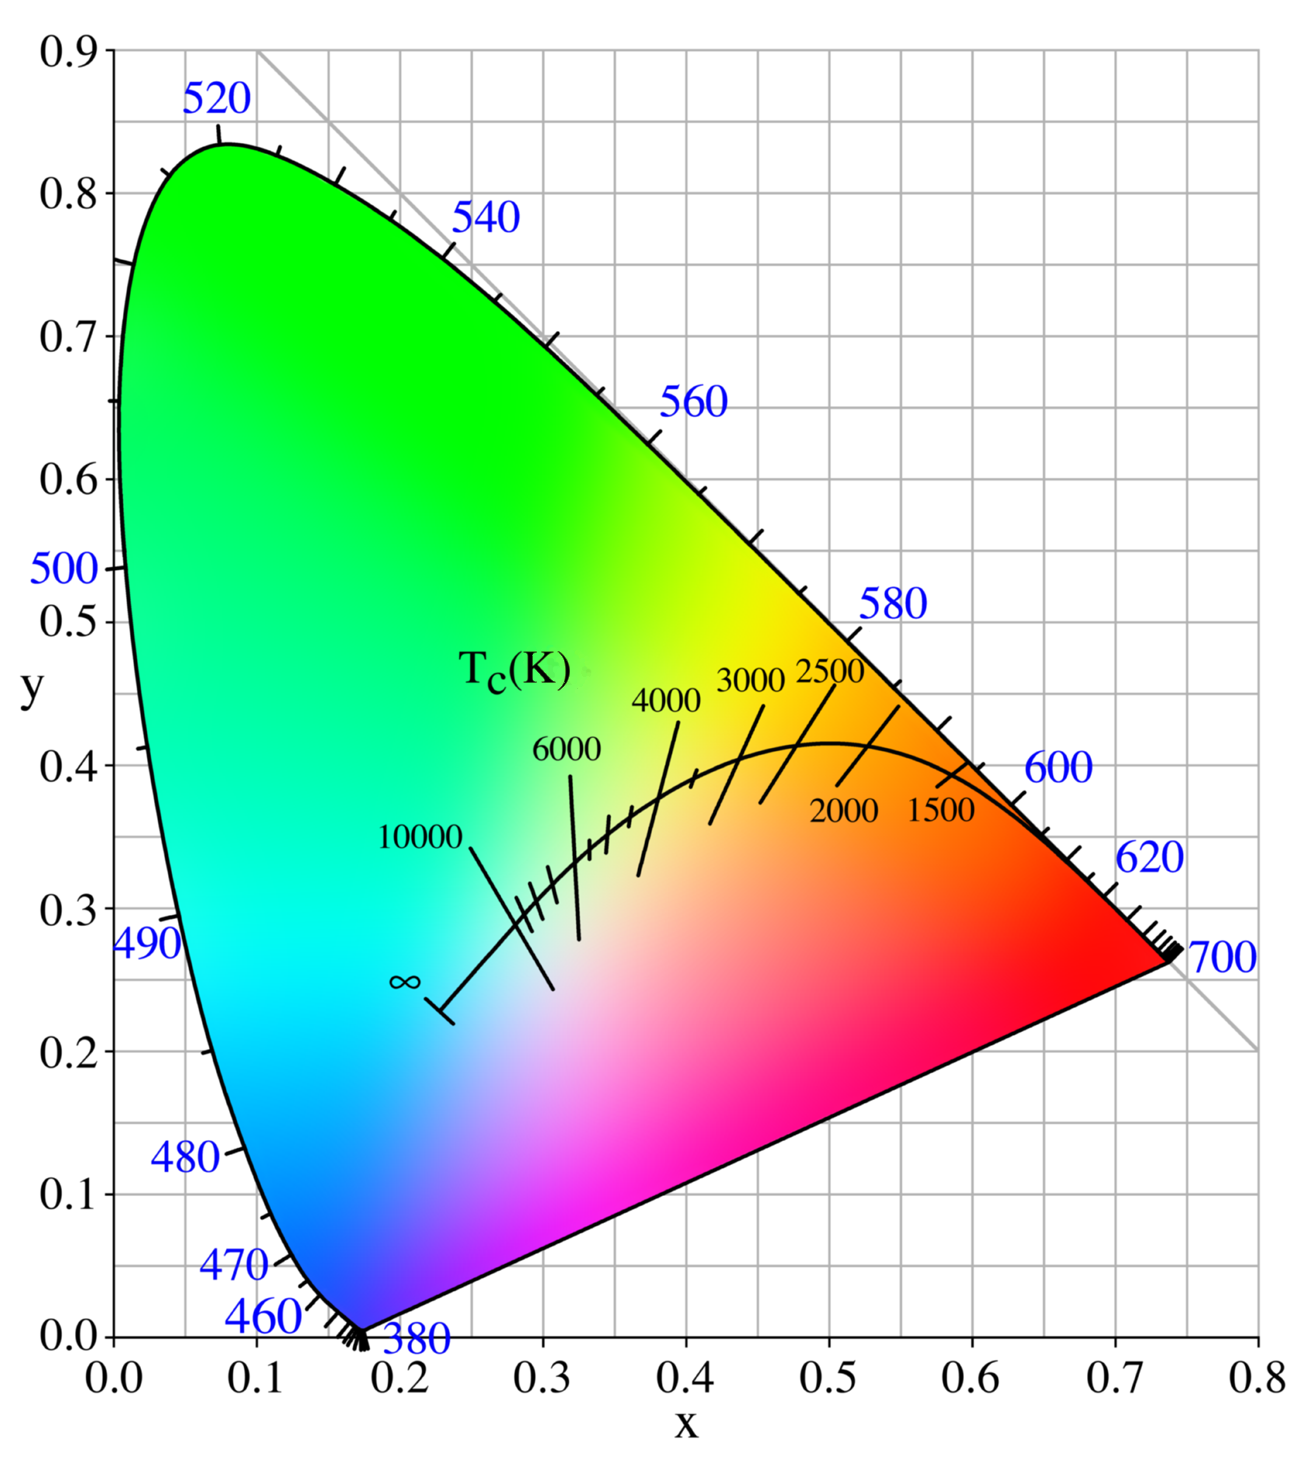
\includegraphics[width=0.6\linewidth]{figs/PlanckianLocus.png}
    \caption{Chromaticiteitsdiagram ~\cite{Chromaticiteit2017}}%
    \label{fig:chromaticiteitsdiagram}
\end{figure}

\subsection{Correlated color temperature}

Een andere belangrijke waarde bij de chromaticiteit is de \gls{cct}. De \gls{cct} is een maat voor de kleur van een lichtbron aan de hand van een temperatuur. Deze maat is gebaseerd op temperaturen bij ''blackbody radiators''. Een ''blackbody radiator'' is een object dat alle invallende straling absorbeert en vervolgens weer uitzendt.

Bij een ''blackbody radiator'' is de kleur volledig afhankelijk van de temperatuur. Hierdoor kunnen we de temperatuur van een ''blackbody radiator'' gebruiken om zijn kleur te beschrijven. Zo bevindt een witte ''blackbody radiator'' zich bijvoorbeeld rond 5000 K.

We kunnen de ''Color temperature'' linken met de chromaticiteit aan de hand van de curve in \cref{fig:chromaticiteitsdiagram}. Deze curve wordt de ''blackbody locus'' of blackbody curve genoemd en stelt de kleur voor van ''blackbody radiators'' bij verschillende temperaturen.

Wanneer de chromaticiteit van een lichtbron op de ''blackbody locus'' ligt, kan de ''Color temperature'' gegeven worden. Ligt de chromaticiteit van een lichtbron echter niet op de ''blackbody locus'', dan kan deze waarde niet worden gebruikt. In dit geval wordt de \gls{cct} waarde gebruikt, die de temperatuur van een ''blackbody radiator'' weergeeft die ongeveer dezelfde kleur heeft als de lichtbron.

\section{Color rendering index}

De \gls{cri} is een maat voor hoe goed een lichtbron kleuren kan weergeven ~\cite{ColorRenderingLight,LightingTechnologyHandbook}. Het is een getal tussen 0 en 100, waarbij 100 de beste kleurweergave voorstelt. De \gls{cri} wordt berekend aan de hand van de kleurweergave van 8 of meer testkleuren.

De \gls{cri} waarde wordt bepaald door de kleursverandering van een testkleur onder de lichtbron te vergelijken met de kleursverandering van de testkleur onder een referentie lichtbron. Van elke van deze 8 of meer kleuren wordt de $R_i$ waarde berekend, wat de kleurverandering van de testkleur onder de lichtbron aangeeft in vergelijking met de referentiebron. Aan de hand van deze $R_i$ waarden wordt een gemiddelde berekend, de \gls{cri} waarde. 

In de standaardmethode is de referentiebron een black body radiator wanneer de \gls{cct} van de lichtbron kleiner is dan 5000K. Is de \gls{cct} groter dan 5000K, dan wordt een mathematisch model van daglicht gebruikt als referentiebron. Naast de acht standaardkleuren kunnen er ook zes extra kleuren optioneel worden toegevoegd. Deze kleuren verbeteren de nauwkeurigheid van de \gls{cri} waarde. 

Van deze extra kleuren is $R_9$ een zeer belangrijke ~\cite{WhatCRIR9}. Lichtbronnen met een lage $R_9$ waarde worden namelijk vaak als onaangenaam ervaren. Dit komt doordat de testkleur voor $R_9$ een rode kleur is, die belangrijk is voor de weergave van bijvoorbeeld huidskleur. Veel lichtbronnen stralen minder licht uit bij de rode golflengtes, waardoor de $R_9$ waarde vaak laag is. Dit is echter niet zichtbaar in de standaard \gls{cri} waarde.

De \gls{cri} waarde is belangrijk voor het beoordelen van de kwaliteit van een lichtbron, maar het is niet altijd de beste maatstaf. De \gls{cri} is niet in staat om lichtbronnen goed te rangschikken, vooral niet wanneer \gls{led}s worden gebruikt. Dit komt door de dunne emissiespectra van \gls{led}s, waarin het licht wordt gemengd. Voor deze reden worden nog andere methodes gebruikt/ontwikkeld om de kleurweergave van lichtbronnen te beoordelen. Het is belangrijk dat deze methodes worden gebruikt als een hulp bij het beoordelen van de kwaliteit van een lichtbron en niet als enige maatstaf.

\subsection{Berekening CRI\texorpdfstring{~\cite{rootPrincipleBasicCalculation,ColorRenderingIndexWiki}}{}}

In de standaardberekening van de \gls{cri} waarde wordt de ''color rendering'' van de testbron vergeleken met die van een referentiebron. Zoals eerder vermeld, wordt een black body radiator als referentiebron gebruikt wanneer de \gls{cct} van de testbron kleiner is dan 5000K. Is de \gls{cct} groter dan 5000K, dan wordt een mathematisch model van daglicht gebruikt.

De berekening begint met het bepalen van de x,y-co\"ordinaten van de testbron. Deze co\"ordinaten worden omgezet naar u,v-co\"ordinaten. De u,v-co\"ordinaten zijn een andere manier om kleuren te representeren en worden vaak gebruikt in kleurwetenschap vanwege hun perceptuele uniformiteit. De u,v-co\"ordinaten worden vervolgens gebruikt om de \gls{cct} te berekenen door het dichtstbijzijnde punt op de Planckian locus te vinden. Aan de hand van deze \gls{cct} waarde wordt de referentiebron bepaald.

Daarna wordt de afstand van de testbron tot de Planckian locus (DC) berekend. Dit geeft aan of het resultaat relevant is. De \gls{cri} waarde is namelijk enkel gedefinieerd voor lichtbronnen die ongeveer wit zijn.

% formula of DC
\begin{align*}
    DC = \sqrt{(u - u_{\text{Planckian}})^2 + (v - v_{\text{Planckian}})^2}
\end{align*}

Als de waarde van DC boven $5.4 \times 10^{-3}$ ligt, is de \gls{cri} waarde niet relevant.

Vervolgens worden de testsamples belicht met zowel de testbron als de referentiebron. Aan de hand hiervan worden de u,v-co\"ordinaten van het licht dat door de testsamples gereflecteerd wordt, bepaald. Daarna wordt op elk van deze samples een von Kries-transformatie toegepast. Dit is een transformatie die wordt uitgevoerd om rekening te houden met ''chromatic adaptation''.

''Chromatic adaptation'' is het fenomeen waarbij de gevoeligheid van de ogen verandert om zich aan te passen aan veranderingen in de lichtbron ~\cite{ChromaticAdaptation2023,LightingTechnologyHandbook}. Dit fenomeen zorgt ervoor dat een object onder verschillende belichtingen grotendeels hetzelfde blijft. Zo zal een appel zelfs onder verschillende lichtbronnen nog steeds rood lijken.

De von Kries-transformatie wordt uitgevoerd aan de hand van de volgende formules:

\begin{align}
    c &= \frac{4.0 - u - 10.0v}{v} \\
    d &= \frac{1.708v - 1.481u + 0.404}{v}\\
    u_{c,i} &= \frac{10.872 + 0.404\left(\frac{c_r}{c_t}\right)c_{t,i} - 4\left(\frac{d_r}{d_t}\right)d_{t,i}}{16.518 + 1.481\left(\frac{c_r}{c_t}\right)c_{t,i} - \left(\frac{d_r}{d_t}\right)d_{t,i}} \\
    v_{c,i} &= \frac{5.520}{16.518 + 1.481\left(\frac{c_r}{c_t}\right)c_{t,i} - \left(\frac{d_r}{d_t}\right)d_{t,i}}
\end{align}

Nu kan voor elk sample de euclidische afstand tussen de co\"ordinaten van de testbron en de referentiebron berekend worden. Ten slotte kan de \gls{cri} waarde berekend worden aan de hand van de volgende formule:

\begin{align}
    R_i = 100 - 4.6\Delta E_i
\end{align}

Met $\Delta E_i$ de euclidische afstand tussen de co\"ordinaten van de testbron en de referentiebron voor de $i$-de sample.

Door het nemen van het gemiddelde van de $R_i$ waarden kan de \gls{cri} waarde berekend worden. Het is echter natuurlijk ook belangrijk deze waarden apart te bekijken.

\section[tm30]{tm30\texorpdfstring{\footnote{Gebaseerd op ~\cite{david2018}.}}{}}


Tm30 is een methode voor het evalueren van lichtbronnen die gebruik maakt van een statistische aanpak. Ze stelt zowel algemene eigenschappen (zoals de gamut area) als hue-specifieke eigenschappen (zoals chroma shift, hue shift, ...) voor. Deze methode probeert niet \"e\"en specifieke waarde te geven die de lichtbron evalueert, maar biedt de gebruiker de benodigde kennis om een keuze te maken op basis van zijn of haar ervaring.

De methode maakt gebruik van 99 \gls{ces}, die op statistische wijze werden gekozen uit 100.000 mogelijke \gls{ces}. Om de kleur voor te stellen, maakt de methode gebruik van een groot aantal berekeningen (50). Afhankelijk van de situatie kunnen bepaalde van deze berekeningen worden gebruikt om een keuze te maken. De belangrijkste berekeningen zijn:

\begin{itemize}
    \item Fidelity index ($R_f$)
    \item Gamut index ($R_g$)
    \item Color Vector Graphic (CVG)
    \item Local chroma shift
    \item Local hue shift
\end{itemize}


\subsection{Fidelity index}

De fidelity index is een waarde die aangeeft hoe goed een lichtbron de kleuren van een referentiebron kan weergeven.

De fidelity index van tm30 wordt berekend door de ''CAM02-UCS'' co\"ordinaten van elke \gls{ces} onder de testbron en de referentiebron te berekenen. Vervolgens wordt het rekenkundig gemiddlede genomen, geschaald met een factor 6.73 en afgetrokken van 100.

\begin{align}
    R_f' = 100 - 6.73 \left[ \sum_{i=1}^{9_{19}} 99 \left( \Delta E_{\text{Jab},i} \right) \right]
\end{align}

Met $\Delta E_{\text{Jab},i}$ de euclidische afstand tussen de ''CAM02-UCS'' co\"ordinaten van de testbron en de referentiebron voor de $i$-de \gls{ces}.

Vervolgens wordt nog een aanpassing van de schaal gedaan zodat geen negatieve waarden bekomen worden.

\begin{align}
    R_f = 10 \ln \left[ \exp \left( \frac{R_f'}{10} \right) + 1 \right]
\end{align}

\subsection{Hue-angle bins}

Voor het berekenen van de volgende waarden worden de \gls{ces} in 16 hue-angle bins verdeeld. Deze bins worden dan gebruikt om de volgende waarden te berekenen. De bins worden bepaald door de a'-b' co\"ordinaten van de \gls{ces} in 16 stukken te verdelen volgens een radiaal patroon zoals in \cref{fig:huebins}. Het a'-b' co\"ordinatenstelsel is een kleurruimte die de kleur van een lichtbron voorstelt. De a'-as staat voor de rood-groen as en de b'-as voor de geel-blauw as.

% figure of bins
\begin{figure}[H]
    \centering
    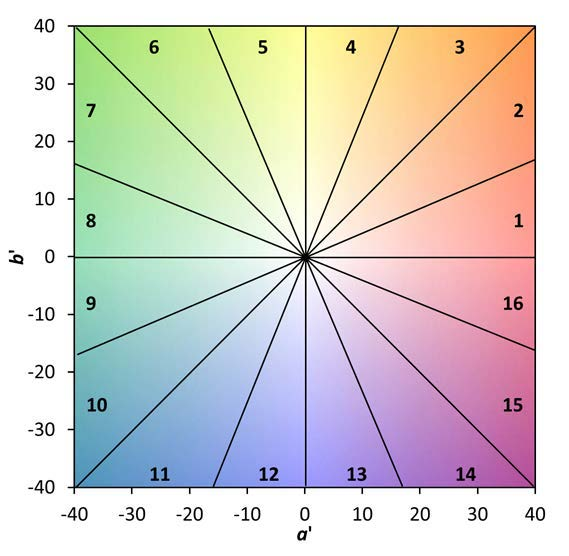
\includegraphics[width=0.6\linewidth]{TM-30-Bins.jpg}
    \caption{Hue-angle bins}%
    \label{fig:huebins}
\end{figure}

\subsection{Gamut (area) index}

De gamut (area) index is een waarde die het gebied aangeeft dat wordt beslagen door de gemiddelde (a', b') co\"ordinaten van de \gls{ces} in elke hue-angle bin. Voor de berekening wordt gewerkt met veelhoeken voor de test- en referentiebron. De gamut index wordt berekend aan de hand van \cref{eq:gamut} met $A_{\text{test}}$ en $A_{\text{ref}}$ als de oppervlakten van de veelhoeken van respectievelijk de test- en referentiebron zoals in \cref{fig:gamut}. ~\cite{david2018,simsWhatGamutArea2022}

\begin{align}
    100 \times \frac{A_{\text{test}}}{A_{\text{ref}}} \label{eq:gamut}
\end{align}

Hiervoor wordt ten eerste voor alle samples het co\"ordinaat van de test en referentiebron berekend zoals in \cref{fig:gamut_samples} voor de testbron te zien is. Vervolgens wordt per bin het gemiddelde van alle test- en referentieco\"ordinaten genomen. Dit levert een veelhoek op voor de test en de referentiebron zoals te zien voor de testbron in \cref{fig:gamut_combined}. Deze veelhoeken worden dan gebruikt om de oppervlakten te berekenen. Aan de hand hiervan kan dan met \cref{eq:gamut} de gamut (area) index berekend worden (\cref{fig:gamut}).

\begin{figure}[H]
    \centering
    \begin{subfigure}[b]{0.45\linewidth}
        \centering
        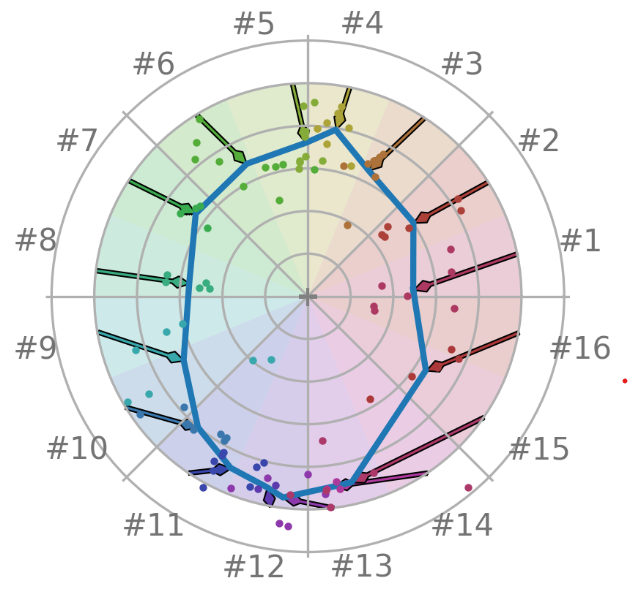
\includegraphics[width=\linewidth]{gamut_samples.png}
        \caption{Test Gamut samples en oppervlak}%
        \label{fig:gamut_samples}
    \end{subfigure}
    \hfill
    \begin{subfigure}[b]{0.45\linewidth}
        \centering
        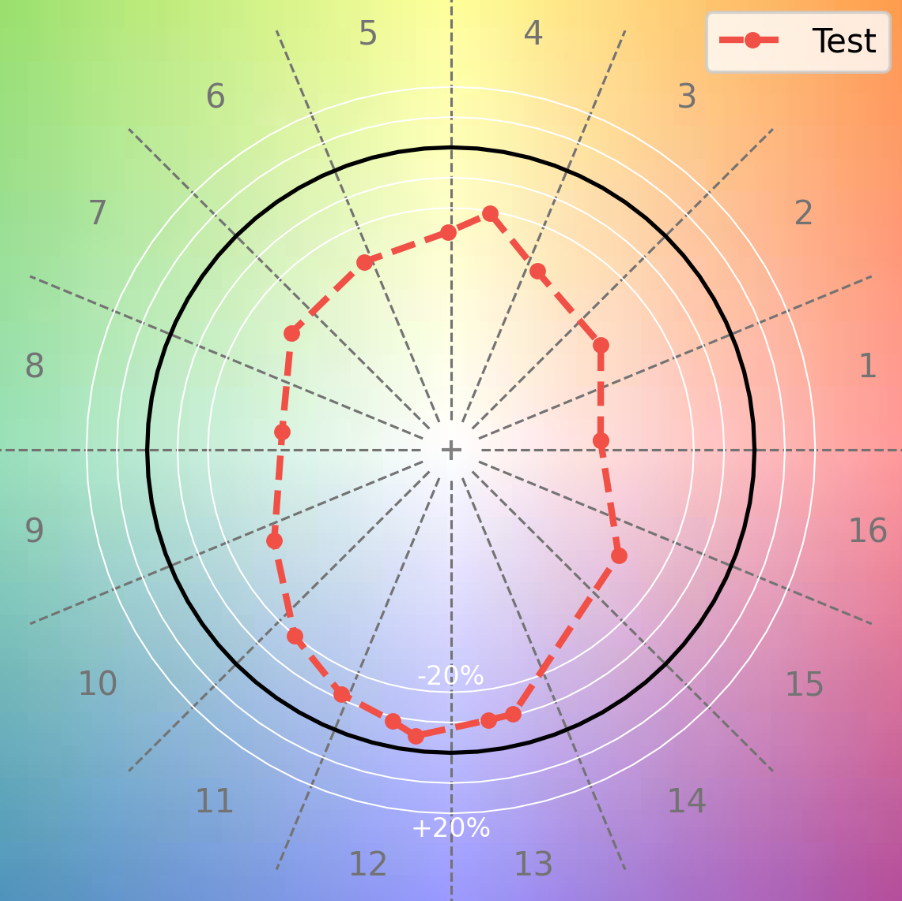
\includegraphics[width=\linewidth]{gamut_index.png}
        \caption{Gamut area index $A_{\text{test}}$ en $A_{\text{ref}}$ (cirkel)}%
        \label{fig:gamut}
    \end{subfigure}
    \caption{Gamut samples (links) en gamut area index (rechts)}%
    \label{fig:gamut_combined}
\end{figure}

\subsection{Color vector graphic}

Een Color Vector Graphic (CVG) laat zien hoe een lichtbron kleuren be\"invloedt. De grafiek toont verschuivingen in kleurintensiteit (chroma) en kleurtint (hue) in een cirkelvormige weergave.

\subsubsection{Chroma (kleurintensiteit)}
\begin{itemize}
    \item Als de lijn van de testlichtbron buiten de referentielijn ligt, worden de kleuren intenser (meer verzadigd).
    \item Ligt de lijn binnen de referentielijn, dan worden de kleuren minder intens (meer dof).
\end{itemize}

\subsubsection*{Hue (kleurtint)}
\begin{itemize}
    \item Als een kleur verschuift langs de cirkel (zonder naar binnen of buiten te gaan), betekent dit dat de tint verandert.
    \item Bijvoorbeeld: een rode tint kan meer oranje worden of juist meer roze.
\end{itemize}

\subsection{Local chroma shift}

De local chroma shift beschrijft hoe de kleurverzadiging lokaal verandert.

\begin{itemize}
    \item Een positieve waarde betekent dat de kleurverzadiging toeneemt (levendiger).
    \item Een negatieve waarde betekent dat de kleurverzadiging afneemt (doffer).
    \item Dit wordt berekend door de gemiddelde chroma van de testlichtbron te vergelijken met de gemiddelde chroma van de referentielichtbron in elk van de 16 hue-angle bins en wordt voorgesteld als een percentage.
\end{itemize}

\subsection{Local hue shift}

De local hue shift beschrijft hoe de kleurtint lokaal verandert.

\begin{itemize}
    \item Een positieve waarde betekent dat de kleurtint verschuift naar een andere kleur tegen de klok in.
    \item Een negatieve waarde betekent dat de kleurtint verschuift naar een andere kleur met de klok mee.
    \item Dit wordt berekend door te kijken naar de tangenti\"ele verplaatsing van de kleuren binnen elk van de 16 hue-angle bins.
\end{itemize}

\section{Luminescente materialen}

Het maken van wit licht vergt zeven kleuren (violet, blauw, groen, geel, oranje, rood en paars). Dit zou dus betekenen dat om wit licht met \gls{led}s te maken er zeven \gls{led}s moeten gebruikt worden.

Er kan echter ook gebruik gemaakt worden van ''Additive color mixing'' om de perceptie van wit licht te cre\"eren. Dit kan gedaan worden door rood, groen en blauw te mengen. Omdat het menselijk oog trichomatric is levert dit een wit licht op. Het grote probleem met het gebruiken van deze ''mixing'' technieken is dat er meerdere \gls{led}s nodig zijn. Dit zorgt voor een grotere kost, het probleem ligt zich hier vooral bij de groene \gls{led} en de eerder vermelde ''green gap''(\cref{sec:external-quantum-efficiency}).

Om dit probleem op te lossen kan gewerkt worden met luminescente materialen zoals fosforen. Hierbij kan een wit licht bekomen worden met slechts \'e\'en \gls{led}. Dit bijvoorbeeld met een blauwe \gls{led} en een gele fosfor.

\subsection{Werking luminescente materialen}

In de meeste materialen wordt geabsorbeerd licht omgezet naar warmte. Bij luminescente materialen wordt een deel van dit licht echter ook omgezet naar licht met een hogere golflengte. In luminescente materialen resulteert de moleculaire structuur in energiebanden met elektronen. Hierbij is er een ''valence'' band waar de elektronen in een stabiele toestand zijn en een ''conduction'' band waar de elektronen vrij kunnen bewegen zoals te zien in \cref{fig:energybands}. De kloof tussen deze twee banden wordt bepaald door de configuratie van de atomen in het materiaal en kan door het toevoegen van onzuiverheden gemanipuleerd worden.

\begin{figure}[H]
    \centering
    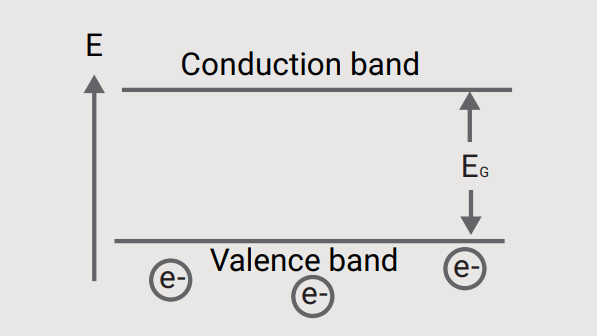
\includegraphics[width=0.6\linewidth]{figs/energy_bands.png}
    \caption{Energiebanden ~\cite{PhosphorModelingLightTools}}%
    \label{fig:energybands}
\end{figure}

Wanneer een luminescent materiaal belicht wordt zullen fotonen van het licht geabsorbeerd worden. Als de energie van de fotonen gelijk is aan het energieverschil tussen de twee banden zal een elektron van de ''valence'' naar de ''conduction'' band springen. De energie van een foton wordt bepaald door de volgende formule:

\begin{align}
E = \frac{hc}{\lambda}\label{eq:energy-foton}
\end{align}
waarbij:
\begin{align*}
h & = \text{Planck's constante} \\
c & = \text{de snelheid van het licht} \\
\lambda & = \text{de golflengte van het licht}
\end{align*}


Na een tijd zal deze elektron terug naar de ''valence'' band vallen. Dit gaat gepaart met het uitgeven van energie in de vorm van licht. In de realiteit zijn er naast deze twee banden nog andere subtoestanden die het toelaten dat een elektron kan verspringen met een lagere hoeveelheid energie. Dit bepaalt het absorptie spectrum van het materiaal.

\begin{figure}[H]
    \centering
    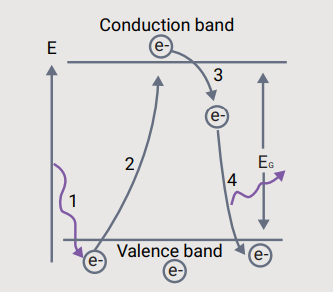
\includegraphics[width=0.6\linewidth]{figs/photolum_process.png}
    \caption{Proces luminescente materialen ~\cite{PhosphorModelingLightTools}}%
    \label{fig:photoluminescent_proc}
\end{figure}

\subsection{Witte LEDs}\label{sec:witte-leds}

Om wit licht te bekomen moeten alle drie de cones in de retina van het oog geactiveerd zijn met een gelijkaardige intensiteit. Dit komt daarnaast overeen met een centrale positie in het chromaticiteitsdiagram. Wit licht kan op een aantal verschillende manieren gegenereerd worden. Zoals eerder vermeld kan dit door kleuren te mengen. Dit kan dichromatic, trichromatic en tetrachromatic (2, 3 of 4 \gls{led}s). Op deze manieren kan een wit licht gegeneerd worden met een hoge \gls{cri} waarde. Er zijn echter veel toepassingen waar de \gls{cri} waarde niet de grootste prioriteit is.

In vele toepassingen is namelijk de efficientie van de lichtbron belangrijker. Om efficient een witte lichtbron te maken met \gls{led}s wordt gebruik gemaakt van luminescente materialen. Aan de hand van deze materialen wordt het licht van een \gls{led} met een bepaalde centrale golflengte omgezet naar licht gecentreerd rond een andere golflengte. Omdat niet al het licht geconverteerd wordt kan zo een witte lichtbron bekomen worden door bijvoorbeeld blauw licht om te zetten naar geel licht.

Naast het feit dat niet al het licht van de \gls{led} geabsorbeerd wordt zijn er ook nog verliezenn bij de omzetting van het licht. Er zijn ten eerste verliezen door de \gls{eqe} van het converterende materiaal.

\begin{align}
\eta_{\text{ext}} = \dfrac{\text{aantal fotonen uitgezonden in vrije ruimte door }\lambda\text{-converter per seconde}}{\text{aantal fotonen geabsorbeerd door }\lambda\text{-converter per seconde}}
\end{align}

Ten tweede treden er ook verliezen op door de conversie naar een hogere golflengte. Dit verschijnsel wordt ook wel de stokes shift genoemd en treed op bij het converteren van een foton met een bepaalde golflengte naar een foton met een hogere golflengte. Deze verliezen trden op omdat de energie van een foton omgekeerd evenredig is met de golflengte (\cref{eq:energy-foton}). Dit betekent dat een foton met een hogere golflengte minder energie heeft dan een foton met een lagere golflengte. Dit verschil in energie wordt omgezet in warmte.

\begin{align}
\Delta E = \frac{hc}{\lambda_1} - \frac{hc}{\lambda_2}
\end{align}

\subsection{Verschillen tussen luminescente materialen}

De verschillende luminescente materialen verschillen van elkaar in absorptie golflengtes, emissie golflengtes, eficientie, excitatie- en emissiespectra. Deze excitatie- en emissiespectra tonen aan hoeveel een luminescent materiaal elektronen naar een hoger niveau brengt en licht emiteerd bij elke golflengte. Het is dan ook logisch dat in bepaalde toepassingen een smal emissiespectrum handiger kan zijn dan een breed emissiespectrum.

\begin{figure}[H]
    \centering
    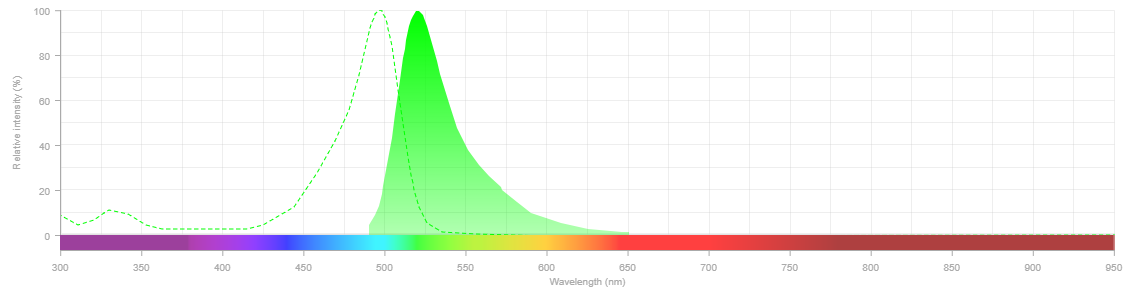
\includegraphics[width=0.9\linewidth]{spectraviewer.png}
    \caption{Emissiespectra (rhodamine 110) ~\cite{FluorescenceSpectraViewer}}%
    \label{fig:rhodamine}
\end{figure}




